\begin{frame}
\frametitle{Data acquired}
\begin{figure}
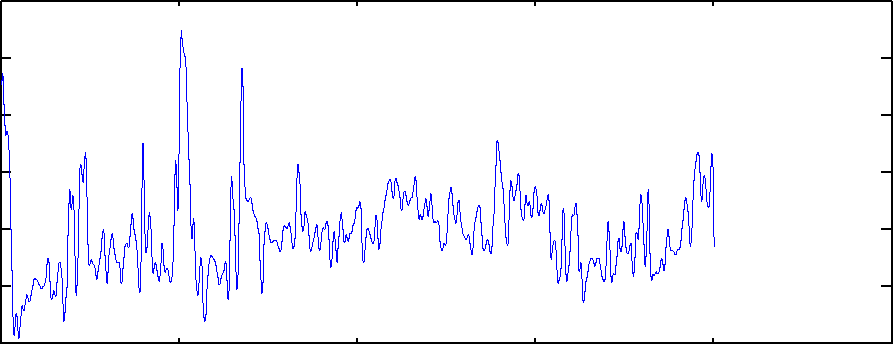
\includegraphics[width=0.6\textwidth]{immagini/gra.png}
\caption{\emph{Output} del codice nel dominio del tempo}
\end{figure}
\begin{figure}
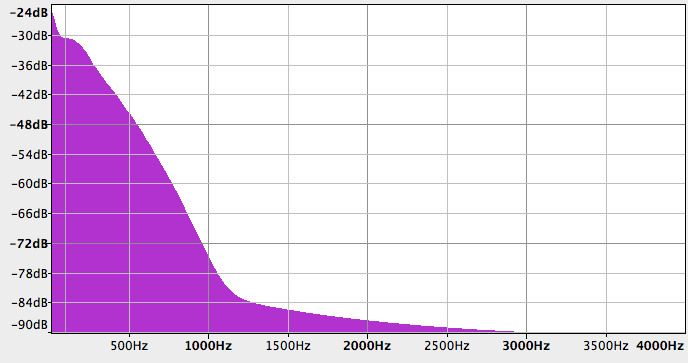
\includegraphics[width=0.6\textwidth]{immagini/freq-domain.png}
\caption{\emph{Output} del codice nel dominio delle frequenze}
\end{figure}
\end{frame}

\begin{frame}
\frametitle{Conclusioni e sviluppi futuri}
\begin{block}{Conclusioni}
Il codice preso in esame termina e risulta solo \emph{parzialmente} utilizzabile.
Una computazione completa su quattro immagini 20096x12576 px ha richiesto 5 giorni su 
un Intel Core 2 Quad con 8 GB di RAM.

%C'\`e ampio spazio per ottimizzazione
\end{block}

\begin{block}{Idee e sviluppi}
\begin{itemize}
\item Definire procedura per la scansione
\item Analizzare algoritmi \emph{a posteriori} per il perfezionamento del centro
\item Valutare diverse strade per il filtraggio del segnale audio grezzo
\item Acquisire traccia con strumenti diversi (lenti, sensori lineari \dots)
\item \dots
\end{itemize}
\end{block}

\end{frame}
